\documentclass[12pt]{article}

\usepackage[a4paper,left=2.5cm,right=2.5cm,top=2.5cm,bottom=2.5cm]{geometry}
\usepackage[bahasa]{babel}

\usepackage{lipsum}
\usepackage{graphicx}
\usepackage{hyperref}
\usepackage{tikz}
% \usepackage{biblatex}
% \addbibresource{main.bib}
\usepackage{apacite}
\usepackage{longtable}
% \usepackage[backend=biber,style=apa,citestyle=apa,sorting=ynt]{biblatex}
% \addbibresource{main.bib}
\usepackage{usebib}
\usepackage{enumitem}

\bibinput{main}
\graphicspath{ {./images/} }
% \title{Tugas SPK}
% \author{Ilman Samhabib 91122010\\62/MMSI/SIB}
% \date{\today}

\begin{document}

% \maketitle
% \titlepage
% \newpage
% \tableofcontents
% \newpage
\begin{center}
   \textbf{Ujian: Testing dan Implementasi Sistem}
%    \\ Tema: \textbf{Ujian}
   \\Ilman Samhabib 9911220\textbf{10} 62/MMSI/SIB

\end{center}

\section*{Soal 1}
Jabarkan kendala-kendala yang mungkin muncul pada saat mengintegrasikan modul-modul software?

\begin{itemize}
    \item keterbatasan \emph{resource} dalam melakukan pengetesan, sehingga akan banyak terjadi \emph{edge cases} yang mungkin tidak diperhitungkan sebelumnya walaupun sebuah tim profesional telah melakukan prosedur yang baik. Nantinya dalam pengintegrasian akan menambah kompleksitas, jika banyak nya \emph{edge cases} yang terjadi.
    \item karena software menggunakan \emph{module module} yang beragam maka akan semakin banyak dan luas hal hal yang harus diverifikasi dan divalidasi, dan kesalahan yang teridentifikasi bisa saja terjadi karena kesalahan modul lain bukan modul yang menjadi objek tahap tes/integrasi tersebut.
    disinilah maka seorang sistem architecture engineer harus dapat menemukan keseimbangan dalam fragmentasi atau seberapa banyak coupling dan decoupling untuk setiap modul modul yang digunakan
    \item modul berbeda harus diberikan \emph{treatment} berbeda dalam pengetesan ataupun integrasi nya, khususnya dalam tool tool dan tingkat kompetensi developer/engineer yang akan terlibat di dalam nya, apalagi jika mengintegrasikan modul open source dari publik repository tanpa melakukan versioning yang tepat, pergantian pada repository publik akan dapat sangat berpengaruh pada software yang tergantung pada modul tersebut. contohnya: \emph{npm dependency cases}, singkat nya banyak modul , maka pengintegrasiannya akan melibatkan tooling dan kompetensi yang lebih kompleks karena semakin banyak nya \emph{moving part}.
\end{itemize}
\section*{Soal 2}
Menurut Saudara bagaimana cara yang baik dalam mengelola sebuah tim dalam pengujian dan pengimplementasian sistem?

\begin{itemize}
    \item  Memilih team yang \emph{fully competent} dalam bidang nya atau dalam hal ini testing dan tool nya, agar teidentifikasi \emph{test cases } yang tepat untuk menjangkau setiap \emph{edge cases}/ hal hal aneh ataupun invalid yang mungkin akan terjadi sebelum \emph{production stage} diterapkan atau dapat memetakan tindakan preventif dari deviasi pada pengoprasian software/sistem informasi ketika implementasi, ini juga berarti personil team yang terlibat dalam pengetesan dan implementasi familiar dengan tool yang digunakan sehingga meningkatkan efisiensi pada saat testing ataupun implementasi
    
    \item Melakukan komunikasi dengan baik dengan \emph{stakeholder} yang dapat berupa rekan se-tim, manager atas, ataupun calon pengguna yang terlibat dalam proses pengujian software, sehingga dapat teridentifikasi bug ataupun improvisasi dan perbaikan yang mungkin hanya dapat dipetakan ketika kita mempunyai prespektif berbeda. Komunikasi yang tidak baik dapat menyebabkan tensi tensi antar personil yang tidak perlu, dan akan menghambat proses pengembangan software/sistem
\end{itemize}


\section*{Soal 3}
Jabarkan tugas yang Saudara kerjakan! \\


Uji Validasi/\emph{validation testing} adalah mengevaluasi suatu sistem dalam mode eksekusi untuk memastikan bahwa sistem tersebut berfungsi dengan  baik pada saat beroperasi nantinya. Untuk memastikan kesiapan perangkat lunak untuk produksi dengan melakukan pengujian yang mengatasi potensi masalah dan penyimpangan dari hasil yang diharapkan. Setiap isu yang teridentifikasi mungkin memerlukan penyesuaian sebelum perangkat lunak diterapkan.

Uji validasi meskipun dengan prosedur yang benar, adalah hal yang sulit dilakukan terutama dalam sistem berskala besar karena kal-hal berikut:
\begin{itemize}
   \item   \textbf{Perangkat Lunak Tidak dalam Mode yang Dapat Diuji:}
         Masalah terkait dengan ketidakmampuan menguji perangkat lunak karena tidak memenuhi kondisi pengujian yang sesuai.
   \item \textbf{Waktu/Sumber Daya yang Tidak Memadai:}
         Keterbatasan waktu atau sumber daya yang dapat mempengaruhi kualitas dan kelengkapan pengujian.
   \item  \textbf{Masalah Signifikan Tidak Terungkap Selama Pengujian:}
         Kekhawatiran bahwa masalah serius mungkin tidak teridentifikasi selama pengujian, yang dapat menyebabkan kesulitan operasional di lingkungan produksi.
\end{itemize}

Semua kegiatan uji validitas haru dimulai dengan Membuat Lingkungan Uji. Sebuah \emph{test environment / workbench} diilustrasikan untuk menjalankan uji dan kemudian mencatat hasil dari uji teresbut, lingkungan diciptakan  sangat  mirip dengan lingkungan pada fase produksi sistem nantinya.
\begin{center}
   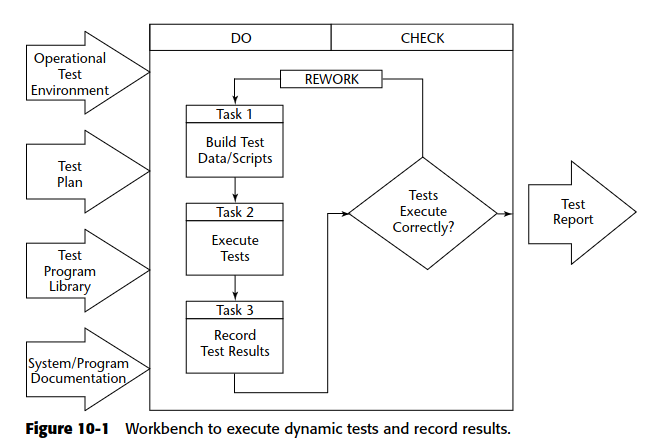
\includegraphics[width=13cm, height=10cm]{images/workbench.png}
\end{center}


Berikut prosedur Melakukan Pengujian Validasi:
Setelah disiapkan \emph{workbench} maka ada 3 langkah yang harus dilakukan selanjutnya:
\begin{enumerate}
   \item Membuat \emph{test data}/data input untuk sistem ketika test dijalankan
   \item Mengeksekusi test, dengan membuat \emph{test cases} untuk hal hal yang mungkin terjadi ketika produksi/implementasi nantinya
   \item Merekam/mendokumentasikan hasil test
\end{enumerate}



% \section*{\emph{Input} Pengujian Validasi:}
% \begin{itemize}
%    \item Masukan untuk pengujian validasi melibatkan rencana uji sistem, data/skrip uji, hasil pengujian verifikasi sebelumnya, dan masukan dari sumber pihak ketiga.
% \end{itemize}

\subsection*{Membangun Data Uji:}
\begin{itemize}
   \item Proses ini melibatkan menciptakan kondisi pemrosesan yang representatif, mempertimbangkan faktor seperti bukti kebenaran, analisis aliran data, dan analisis aliran kontrol.
   \item Berbagai sumber yang dapat dijadikan parameter dalam membuat test data, seperti: dokumentasi sistem, kasus pengguna, generator uji, data produksi, basis data, dan profil operasional.
   \item Penguji harus akrab dengan standar departemen TI untuk merancang file data uji yang memadai, termasuk berbagai data valid dan tidak valid.
   \item Penguji juga harus dapat mengimajinasikan apa output sistem dari setiap input test data yang dirancang tersebut
\end{itemize}

\subsection*{Eksekusi Test}

Persiapan sangat penting untuk menghindari pengujian yang tidak ekonomis dan tidak efektif. Metode yang dapat dijalankan adalah:
\begin{itemize}
   \item \textbf{Pengujian Manual, Regresi, dan Fungsional:}
         \begin{itemize}
            \item Pengujian manual memastikan interaksi pengguna yang benar.
            \item Pengujian regresi memverifikasi dampak instalasi baru pada aplikasi yang sudah ada.
            \item Pengujian fungsional memastikan persyaratan sistem terpenuhi dalam berbagai keadaan.
         \end{itemize}

   \item \textbf{Pengujian Fungsional dan Regresi (Integrasi):}        Memastikan komunikasi yang benar dengan sistem aplikasi terkait.


   \item \textbf{Pengujian Kepatuhan:}
         \begin{itemize}
            \item Termasuk pengujian otorisasi untuk memverifikasi implementasi aturan dengan benar.
            \item Pengujian kinerja, keamanan, integritas file, jejak audit, pengujian kebenaran adalah hal yang penting.
         \end{itemize}

   \item \textbf{Pengujian Pemulihan (Kelangsungan):}  Menguji prosedur alternatif untuk downtime sistem.
         

   \item \textbf{Pengujian Stres (Tingkat Layanan):} Memvalidasi kinerja sistem dalam pemrosesan berkecepatan tinggi.
      

   \item \textbf{Kepatuhan Metodologi:}         
          Pengujian harus mematuhi kebijakan, prosedur, dan dokumentasi yang ditentukan oleh organisasi.
         

   \item \textbf{Pengujian Dukungan Manual (Kemudahan Penggunaan):} Mengevaluasi kegunaan sistem dalam lingkungan yang realistis.
         

   \item \textbf{Inspeksi (Maintainability):}
          Melibatkan inspeksi independen untuk menguji kemampuan pemeliharaan sistem.
         

   \item \textbf{Pengujian Bencana (Portabilitas):}
          Mensimulasikan masalah untuk menguji lingkungan pemrosesan alternatif.
         

   \item \textbf{Pengujian Operasional (Kemudahan Operasi):}
          Dilakukan oleh staf operasional normal untuk menilai keberoperasian sistem tanpa bantuan pengembang.
         
\end{itemize}
Dalam penerapannya ini dilakukan oleh script yang mendefinisikan tiap-tiap \emph{test case} yang sebaiknya mencakupi metode metode diatas, dan dilakukan secara otomatis.



\subsection*{Dokumentasi Hasil Test}
Pendokumentasian hasil uji validasi, dengan merinci atribut kunci untuk setiap kasus uji: 

\begin{enumerate}
   \item Kondisi (apa adanya) .
   \item Kriteria (apa seharusnya). 
   \item Efek (mengapa perbedaan itu signifikan), 
   \item Penyebab (alasan deviasi). 
   
\end{enumerate}
maka Setiap \emph{test case} akan terdokumentasi hal-hal berikut, yang dapat digunakan untuk pemechan masalah:
\begin{itemize}
   
   \item Dokumentasi Deviasi:  Ini melibatkan deskripsi kondisi saat ini (kondisi) dan kriteria yang diinginkan. Deviasi adalah kesenjangan antara kedua keadaan ini.
   
   \item Dokumentasi Efek: Efek menentukan signifikansi dari pernyataan masalah.
   
   \item Dokumentasi Penyebab: Mengidentifikasi penyebab masalah mungkin memerlukan penyelidikan. Penyebab umum termasuk ketidaksesuaian dengan standar, instruksi yang diterbitkan, praktik bisnis yang diterima secara umum, atau praktik yang tidak efisien.
   
\end{itemize}

\end{document}